\section{Stato dell'arte}
\label{sec:stato-arte}
In questa sezione verrà descritto prima lo stato dell'arte dei modelli di evacuazione da tsunami, senza focalizzarsi sui modelli di inondazione,
e successivamente un approfondimento sulla gestione della velocità per i pedoni nel caso di modelli network-based.

I primi modelli di evacuazione da tsunami sono stati basati sui modelli network-based utilizzati per l'evacuazione da altri disastri come
uragani, incendi e inondazioni \parencite{usuzawa1997development, imamura2001development}.

Uno dei primi aspetti che è stato preso in considerazione è il comportamento umano,
in particolare le reazioni dei residenti all'arrivo dello tsunami
e il tempo che ci mettono per iniziare a evacuare.
%
Queste informazioni sono state raccolte tramite dei questionari rivolti ai residenti
e usate per stimare i tempi di partenza dell'evacuazione \parencite{imamura2001development, saito2004simulation}.

Questi primi modelli network-based hanno usato come regola di \textit{path finding}
proseguire verso il nodo con altitudine maggiore.
Successivamente si è passati a usare il percorso
più breve \parencite{katada2004disaster} e altre strategie di routing basate sull'apprendimento 
come Nash equilibrium e system optimal \parencite{lammel2009towards}.

Un altro aspetto importante per l'evacuazione è la conoscenza dell'ambiente da parte degli agenti.
Alcuni lavori hanno distinto gli agenti in base alla loro conoscenza e
studiato gli effetti di diverse proporzioni tra categorie di agenti.
\textcite{nguyen2012simulation} hanno definito \textit{fox agent} un pedone ben informato che segue i segnali
stradali fino a un rifugio e \textit{sheep agent} un pedone che non sa
come comportarsi e quindi segue i \textit{fox agent} o si muove casualmente.
\textcite{takabatake2017simulated} invece hanno distinto gli agenti in residenti e visitatori.
I residenti sono agenti che conoscono il percorso più breve per evacuare, mentre i visitatori
seguono gli altri scegliendo la strada con più individui o si muovono verso una zona più elevata.

Con l'aumento della potenza di calcolo è stato possibile passare da modelli network-based a modelli grid-based e ibridi.
Inoltre è stato possibile usare una quantità di dati maggiore e sfruttare il calcolo parallelo \parencite{wijerathne2013hpc, makinoshima2018enhancing}.

\textcite{wijerathne2013hpc} hanno proposto un modello grid-based che utilizza un sistema di navigazione basato
sulla visione. Gli agenti si muovono verso un luogo sicuro ben visibile scegliendo la strada con una maggiore distanza di visione.
%
Anche in questo lavoro vengono distinti visitatori, che si affidano alla visione, e non-visitatori, che hanno conoscenza di un'area
limita al di fuori della quale vengono considerati visitatori.

% Un altro modello grid-based è quello di \textcite{mas2012agent} 
% in cui è stato proposto un modello di evacuazione statica che da un insieme di informazioni % TODO: specificare (dati demografici, morfologia del terreno, distribuzione della popolazione, ...)
% calcola una mappa dei tempi di evacuazione

% Altri lavori hanno analizzato come i tempi di partenza influenzano il tempi di evacuazione e il numero di vittime
% \parencite{wang2016agent, takabatake2017simulated}.

% Successivamente i modelli di evacuazione da tsunami si sono concentrati sulle applicazioni come trovare delle contromisure, 
% il miglioramento delle modalità di evacuazione
% tramite l'analisi delle congestioni del traffico, il posizionamento dei rifugi e lo scambio di informazioni durante l'evacuazione.
% \parencite{taubenbock2013risk} %TODO: aggiungere citazioni

In molti modelli vengono considerati esclusivamente solo pedoni, ma alcuni lavori hanno analizzato l'aggiunta della presenza di auto e altri veicoli,
e si concentrano nella gestione delle interazioni tra i diversi tipi di agenti.

\textcite{goto2012tsunami} hanno considerato gli individui raggruppati in famiglie e categorizzato le famiglie in:
pedoni lenti, pedoni normali, motociclisti e occupanti di un'auto, gestendo le loro velocità in base alla densità e inoltre hanno
modellato le interazioni dei diversi agenti all'interno di una corsia stradale.

\textcite{wang2016agent} hanno proposto un modello in cui auto e pedoni evacuano separatamente e vengono gestite esclusivamente interazioni auto-auto. Ai pedoni viene assegnata
una velocità costante tramite una distribuizione normale che comprende diversi range di velocità dei pedoni.

\textcite{wang2021novel} hanno ripreso il lavoro di \textcite{wang2016agent} e, 
ispirandosi al lavoro \textcite{goto2012tsunami}, modificato la gestione delle interazioni proponendo un modello in cui sia pedoni che auto hanno una velocità variabile in base alla densità.
Vengono distinti diversi stati di traffico in base al rapporto tra il volume dei pedoni e delle auto: \textit{vehicle-dominated}, \textit{balanced}, e \textit{pedestrian-dominated}. 
Inoltre per rendere il modello più realistico sono stati considerati i danni sulla rete stradale causati dal terremoto che si verifica prima dello tsunami.

\subsection{Velocità dei Pedoni}
La velocità dei pedoni solitamente viene gestita tramite relazioni macroscopiche tra velocità-densità-flusso
espresse tramite un diagramma fondamentale \parencite{nikolic2016probabilistic}.
Per estrarre queste relazioni sono richiesti dei dati empirici che non sempre disponibili, soprattutto nei casi di emergenza.

Perciò analizzeremo come questo problema viene trattato da metodi allo stato dell'arte per la simulazione di evacuazione di tsunami.

Alcuni lavori distinguono i pedoni in gruppi in base alla loro velocità sulla base di questionari o di altri lavori riguardanti il comportamento dei pedoni.
\textcite{takabatake2017simulated} hanno effettuato una distinzione sull'età con una velocità massima di 1.19 m/s (Under 65) e 0.96 m/s (Over 65).
Basandosi sul lavoro di \textcite[]{older1968movement} hanno assunto una decrescità lineare della velocità da un livello di densità di 0.3 p/m² a uno di 3.0 p/m² (Fig. \ref{fig:speed-linear}).
\textcite{goto2012tsunami}, invece hanno raggruppato i pedoni in famiglie che sono distinte in \textit{normal walkers}, con velocità massima di 1.5 m/s, e
\textit{slow walkers} (famiglie con disabili o anziani), con velocità massima di 0.75 m/s (Fig. \ref{fig:speed-goto}).

Altri lavori hanno assunto che la velocità sia distribuita normalmente.
\textcite{wang2021novel} hanno considerato una distribuzione normale $\mathcal{N}(\mu_p,\sigma_p)$ troncata tra 0.75 m/s e 3.83 m/s e
con $\mu_p \sim \mathcal{U}(1.4, 2)$ e $\sigma_p \sim \mathcal{U}(0.1, 0.6)$.

\begin{figure}[ht]
    \centering
    \begin{subfigure}{0.45\textwidth}
        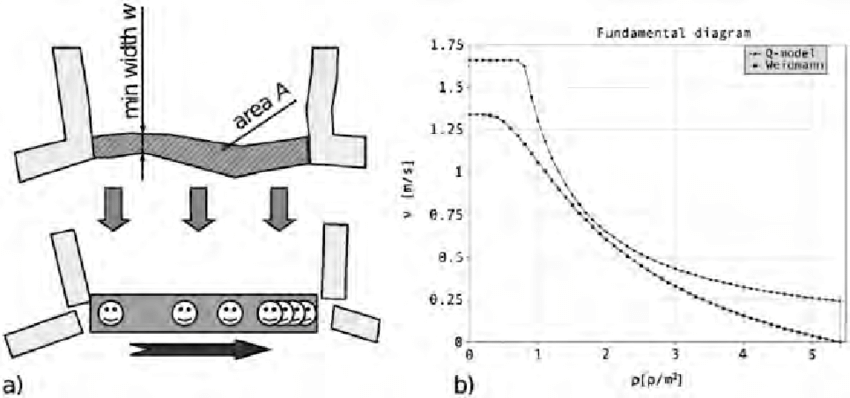
\includegraphics[width=\textwidth]{images/speed_lammel.png}
        \caption{}
        \label{fig:speed-lammel}
    \end{subfigure}
    \hfill
    \begin{subfigure}{0.45\textwidth}
        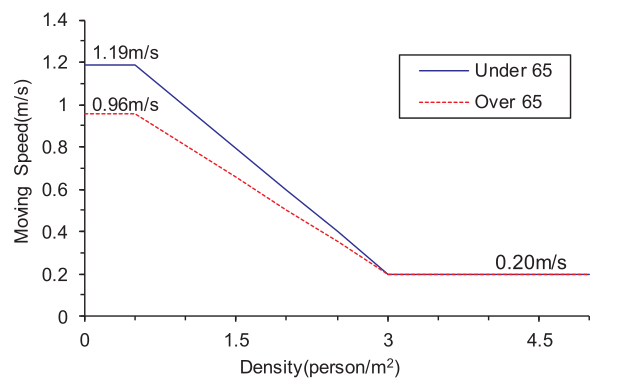
\includegraphics[width=\textwidth]{images/speed_Linear.png}
        \caption{}
        \label{fig:speed-linear}
    \end{subfigure}
    \begin{subfigure}{0.45\textwidth}
        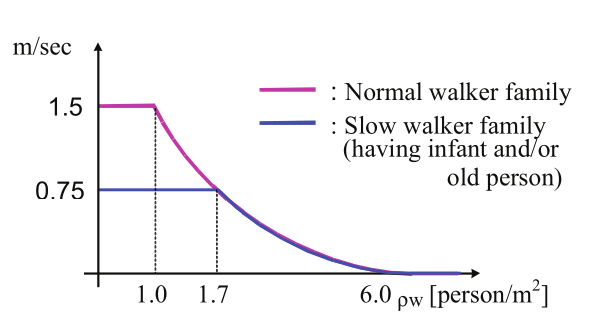
\includegraphics[width=\textwidth]{images/speed_GOTO.png}
        \caption{}
        \label{fig:speed-goto}
    \end{subfigure}
    \hfill
    \begin{subfigure}{0.45\textwidth}
        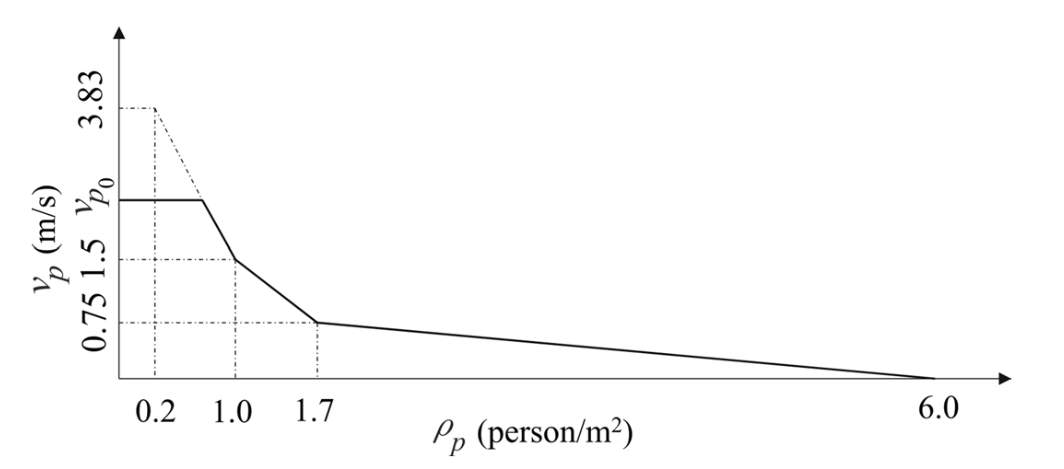
\includegraphics[width=\textwidth]{images/speed_WANG.png}
        \caption{}
        \label{fig:speed-wang}
    \end{subfigure}
    \caption{Relazione velocità-densità.
        a) \textcite[]{lammel2010emergency},
        b) \textcite[]{takabatake2017simulated},
        c) \textcite[]{goto2012tsunami},
        d) \textcite[]{wang2021novel}.
    }
    \label{fig:speeds}
\end{figure}

In questi lavori la velocità viene aggiustata in base alla densità in un'area davanti ai pedoni (Fig. \ref{fig:speeds}), tramite la seguente formula
$\rho = n /(L \times W)$, dove $n$ è il numero di persone nell'area $L \times W$, $L$ è la lunghezza di ricerca, che assume solitamente assume valori tra 3 e 5 m, e $W$ la larghezza della strada.

\textcite{lammel2010emergency} invece hanno introdotto un modello network-based in cui in ogni link viene assegnata una coda FIFO,
limitata nel flusso in uscita \textit{flow capacity} e nella capacità di pedoni al suo interno \textit{storage capacity}.

La velocità viene aggiornata tramite la relazione $v = \min[v_{max}, FC / D]$ (Fig. \ref{fig:speed-lammel}),
dove $D$ la densità e $FC$ è la \textit{flow capacity}.
i parametri di tale modello sono stati scelti approssimando la curva velocità-densità del modello a code a quella
del diagramma fondamentale di \textcite{weidmann1993transporttechnik}.
Inoltre è stata considerata una velocità massima di 1.66 m/s poichè i valori considerati da Weidmann sono relativi
al flusso dei pedoni in condizioni normali e non in caso di emergenza.

% \vspace*{5mm}
% [Lammel 2010] modello a code FIFO(first-in first-out) con tre restrizioni:
% Primo ogni agente deve restare su un link per un determinato tempo ovvero il free flow speed travel time.
% Secondo una Flow capacity capacità sul flusso del link è definita che ne limita il flusso in uscita.
% Infine una Storage capacity che limità il numero di pedoni che possono stare sul link viene definità.

% \begin{equation}
%     v = min [v_{max}, FC / D]
% \end{equation}

% La seguente equazione mostra il diagramma velocità densità prodotto dal modello, dove FC (Flow capacity) 
% è stato scelto in modo da approssimare il diagramma fondamentale di Weidmann (Weidmann, 1993).
% Inoltre $v_{max}$ è più alta.

% La densità è calcolata ad ogni step considerando gli agenti a 5m di distanza e la larghezza della strada. 
% La densità viene definità come density ahead $\rho_w = n/(Lw x W )$, dove n: numero di persone in Lw x W area,
% Lw : search length (3 m), W : road width.

% Basato sulla speed-density relationship in Goto et al (2012), introduce un modello di aggiustamento della velocità dei pedoni
% come mostrato in figura \ref*{fig:speed-WANG}, dove vp0 rappresenta la free flow speed e $\rho_p$ la density ahead dei pedoni con search length di 4m.

% Come appena descritto i lavori analizzati, apparte avere informazioni sull'eta e sulle velocità massime dei pedoni, non hanno dati a loro disposizione per fittare i modelli.
% Di conseguenza non avendo dati empirici per questo lavoro si è deciso di usare il diagramma fondamentale di \textcite{weidmann1993transporttechnik},
% il quale descrive la relazione tra densità e velocità tramite la Kladek-formula (Eq. \ref{eq:kladek-formula}),
% dove $v_{f}$ è la free flow speed mentre $\rho$ è la densità e $\rho_{max}$ è la jam density.
% %
% \begin{equation}
%     v = v_{f} \times (1 - e^{-\gamma \times (\frac{1}{\rho} - \frac{1}{\rho_{max}})})
%     \label{eq:kladek-formula}
% \end{equation}

% I parametri scelti sono $\gamma = 1.913$, $v_f = 1.34$ m/s and $\rho_{max} = 5.4$ p/m² che secondo studi empirici hanno mostrato i risultati migliori.
